\documentclass[9pt]{beamer}

% \usepackage{beamerthemesplit} // Activate for custom appearance
\usepackage{geometry,hyperref, url, amsmath, amssymb,graphicx}
\usepackage{amsthm}
\usepackage{tikz}
\usepackage{mathtools}
\usepackage{mathrsfs} %mathscr dans beamer
\usepackage{algorithm}
\usepackage{algpseudocode}
\usepackage{amsmath}
\usepackage[utf8]{inputenc}
\usepackage[T1]{fontenc}
\usepackage[english]{babel}
\usepackage{booktabs}
\usepackage{subcaption}
\usepackage{siunitx}
\usepackage{booktabs}
\usepackage{multirow}
\usepackage{gensymb}

% \qty should normally used to typeset SI quantities, but since it is already defined by the physics package, we need to use \SI
\sisetup{separate-uncertainty}
\sisetup{per-mode=fraction}
\usepackage{multirow}

\usepackage{hyperref}
\hypersetup{colorlinks = true, urlcolor = black, linkcolor = black, citecolor = black}
\usetikzlibrary{babel}

\usepackage{lmodern}% http://ctan.org/pkg/lmodern
\usepackage{slantsc}% http://ctan.org/pkg/slantsc
\newcommand{\instbit}[1]{\mbox{\scriptsize #1}}
\newcommand{\instbitrange}[2]{~\instbit{#1} \hfill \instbit{#2}~}
\usetheme{Warsaw}
\usefonttheme{serif}
\usecolortheme{crane}%crane spruce
\setbeamertemplate{navigation symbols}{}
\setbeamertemplate{footline}{}



\setbeamertemplate{footline}[frame number]  %numbers the slides


\definecolor{clarblue}{rgb}{0.501803,0,0.7843137}
\definecolor{lightred}{rgb}{1,0.2235294118,0}
\definecolor{heavyred}{rgb}{0.3803921569,0,0}
\definecolor{gold}{RGB}{252,187,6}
\definecolor{yg}{RGB}{249,234,183}
\definecolor{lightgreen}{RGB}{197,223,117}
\definecolor{lightblue}{RGB}{153,217,234}
\definecolor{darkgreen}{RGB}{50, 180, 50}
\definecolor{lightbrown}{RGB}{210, 170, 149}
\definecolor{verylightgray}{RGB}{210, 210, 210}
\definecolor{deepblue}{RGB}{0, 111, 157}
\definecolor{sky}{RGB}{57, 146, 236}
\definecolor{sky2}{RGB}{90, 163, 242}


\newtheorem{defi}{Definition}[section]
\newtheorem{theo}{Theorem}[section]
\newtheorem{exemple}{Example}[section]
\newtheorem{rem}{Remark}[section]


\renewcommand{\tablename}{\textsc{Table}}



\setbeamercolor{section in toc}{fg=black}
\setbeamerfont{section in toc}{shape=\scshape}
\setbeamercolor{section number projected}{bg=gold,fg=black}
\setbeamercolor{subsection number projected}{bg=gold,fg=black}
\setbeamercolor{item projected}{bg=black,fg=gold}

\DeclareMathOperator{\ones}{ones}
\DeclareMathOperator{\diag}{diag}
\DeclareMathOperator{\som}{sum}
\DeclareMathOperator{\tr}{Tr}

% New commands and shortcuts
\renewcommand{\leq}{\leqslant}
\renewcommand{\geq}{\geqslant}
\newcommand{\ms}[1]{\mathscr{#1}}
\renewcommand{\eqref}[1]{eq. (\ref{#1})}
\newcommand{\figref}[1]{\textsc{Figure} \ref{#1}}
\newcommand{\tabref}[1]{\textsc{Table} \ref{#1}}


\newcommand{\Phx}{\Phi_x}
\newcommand{\Phy}{\Phi_y}
\newcommand{\X}{\mathcal{X}}
\newcommand{\Y}{\mathcal{Y}}
\newcommand{\C}{\mathcal{C}}
\newcommand{\I}{\mathcal{I}}
\newcommand{\U}{\mathcal{U}}
\newcommand{\R}{\mathbb{R}}
\newcommand{\N}{\mathbb{N}}
\newcommand{\E}{\mathbb{E}}
\renewcommand{\P}{\mathbb{P}}
\renewcommand{\H}{\mathscr{H}}
\newcommand{\G}{\mathscr{G}}
\newcommand{\fat}{f_\theta^a}
\newcommand{\fbt}{f_\theta^b}
\newcommand{\norm}[1]{\left\|#1\right\|}
\newcommand{\nhs}[1]{\left\|#1\right\|_\text{HS}}
\newcommand{\scal}[2]{\left\langle #1 \vert #2 \right\rangle}
\usepackage{natbib}


%\logo{\includegraphics[height=1cm]{logo.png}} % inserts the logo
%\insertlogo %to insert

%title slide parameters

%\title{ \\ }
%\subtitle{}
\author{\\
\textsc{Pierre Cornilleau}\\
\textsc{Abel Douzal} \\
 \textsc{Ruben Ifrah}}
\date{}


%title slide
\setbeamertemplate{title page}{
  \begin{center}
    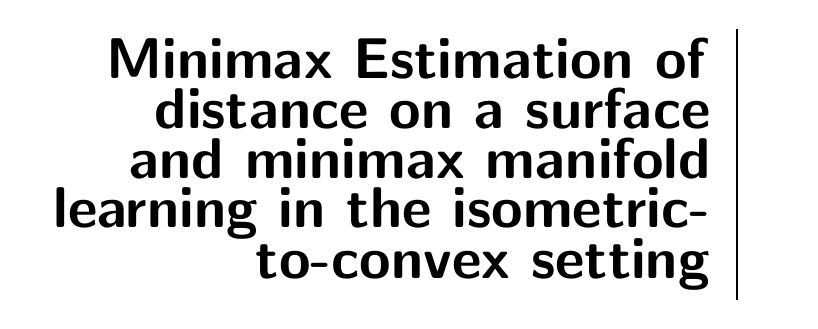
\begin{tikzpicture}
        \draw (0, 0) node(T)[anchor=north east]{\sffamily\begin{tabular}{r}
            %\Large\inserttitle \medskip\\
            \huge\textbf{Minimax Estimation of}\\
            \huge\textbf{distance on a surface}\\
            \huge\textbf{and minimax manifold}\\
            \huge\textbf{learning in the isometric-}\\
            \huge\textbf{to-convex setting}\\
            %\Large\textbf{\insertsubtitle}\\
        \end{tabular}};
        \draw[thick] (T.north east) -- (T.south east) node[midway, anchor=west]{
          \begin{tabular}{l}
            \Large\insertauthor\\
            \Large\insertdate
          \end{tabular}};
    \end{tikzpicture}\vspace{1cm}\\
    \textit{Dauphine PSL -- ENS-PSL  -- École polytechnique}\\
  \end{center}
}

\AtBeginSection[]{
  \begin{frame}<beamer>{Outline}
    \tableofcontents[currentsection]
  \end{frame}
}


\begin{document}


\frame{\titlepage}
\frame{\tableofcontents}

\section{Introduction}
\frame{\frametitle{Main goals}
\textbf{Setting:} 
given a finite set of points $\{x_i\}_{1\leq i\leq n}$ on $\mathcal{M}$ a $\mathscr{C}^2$ $d$-submanifold,
\begin{itemize}
    \item Non parametric estimation of intrinsic distances $d_\mathcal{M}(x_i, x_j)$
    \item Application in Manifold learning (i.e. dim reduction)
    \item Main non-parametric hypothesis :
    $$\max_{x\in\mathcal{M}} \min_{1\leq i \leq n} \norm{x-x_i} \leq \varepsilon $$
    \item Anterior bound for $\mathscr{C}^2$ submanifolds gives a relative error rate in $O(\varepsilon^{2/3})$ :
    $$\left| d_\mathcal{M}(x_i, x_j) - \widehat{d}_{ij} \right| \leq C \varepsilon^{2/3} d_\mathcal{M}(x_i, x_j)$$
\end{itemize}
}


\section{Main result}
% \frame{\centering{\Large{\textsc{Main Result}}}}
\frame{\frametitle{Main result (Arias-Castro \& Chau)}
Nota : for $n$ points on $\mathcal{M}$, we have at best  $\varepsilon \asymp ((\log n)/n)^{1/d}$.

\medskip

\textbf{Main results}
\begin{enumerate}
    \item \textbf{A Minimax Optimal Rate:} They prove that the theoretical optimal error rate for geodesic estimation is exactly quadratic in the sampling density $O(\varepsilon^2)$:
    $$\left| d_\mathcal{M}(x_i, x_j) - \widehat{d}_{ij} \right| \leq C \varepsilon^{2} \min (d_\mathcal{M}(x_i, x_j), \widehat{d}_{ij})$$
    \item \textbf{Constructive Attainment:} This minimax rate cannot be attained by 1D graphs, but it \textit{is} attained by geodesic paths calculated across the flat faces of a reconstructed mesh (Tangential Delaunay Complex).
\end{enumerate}
% \end{frame}

\medskip

}






\frame{\frametitle{Proof global structure for minimax bound in two parts}

\textbf{1. Upper bound (non constructive):} \\
Prove $|d_{\mathcal{M}}(x,y) - \widehat{d}(x,y)| / d_{\mathcal{M}}(x,y) \lesssim \varepsilon^2$ using:
\begin{itemize}
    \item Axiom of choice,
    \item Geodesic stability on nearly-isometric surfaces.
\end{itemize}

\medskip

\textbf{2. Lower bound (information-theoretic):}
\begin{itemize}
  \item Construct two manifolds with geodesic distances differing by $O(\varepsilon^2)$ that are statistically indistinguishable from $n$ samples.
  \item No estimator can achieve better than $O(\varepsilon^2)$ worst-case error.
\end{itemize}

\medskip

\textbf{Key limitation:} The $\varepsilon^2$ distortion is fundamental—intrinsic to the sampling resolution, not the algorithm.

}



% \frame{\frametitle{TDC}
% une méthode qui atteint les taux minimax.

% expliquer plus en détail potentiellement
% }



\begin{frame}{Tangential Delaunay Complex (TDC)}

\textbf{Motivation:} Need a provably good mesh reconstruction of $\mathcal{M}$ from point samples to compute geodesics.

\medskip

\textbf{Why TDC?} Only known method simultaneously guaranteeing:
\begin{enumerate}
  \item \textbf{Correct topology:} TDC is homeomorphic to $\mathcal{M}$ when $\varepsilon < \mathrm{reach}(\mathcal{M})/2$.
  
  \item \textbf{Geometric fidelity:} Hausdorff distance $d_H(\text{TDC}, \mathcal{M}) = O(\varepsilon^2)$.
  
  \item \textbf{Geodesic stability:} Polyhedral geodesics on TDC approximate $d_{\mathcal{M}}$ with relative error $O(\varepsilon^2)$.
\end{enumerate}

% \medskip

% \textbf{Why TDC achieves minimax rates:} It's the only known reconstruction that simultaneously guarantees correct topology \emph{and} $O(\varepsilon^2)$ metric distortion.

\end{frame}
% \frame{\frametitle{Tangential Delaunay Complex (TDC)}

% \textbf{Motivation:} Need a provably good mesh reconstruction of $\mathcal{M}$ from point samples to compute geodesics.

% \medskip

% \textbf{Construction (Aamari--Levrard):}
% \begin{enumerate}
%   \item For each sample point $x_i$, estimate the tangent space $T_{x_i}\mathcal{M}$ (e.g., via local PCA on $k$-nearest neighbors).
%   \item Build the \textit{Tangential Delaunay complex}: triangulate points using Delaunay criterion restricted to their estimated tangent spaces.
%   \item Output: a simplicial complex approximating $\mathcal{M}$.
% \end{enumerate}

% \medskip

% \textbf{Key properties:}
% \begin{itemize}
%   \item \textbf{Topological correctness:} TDC is homeomorphic to $\mathcal{M}$ when $\varepsilon < \mathrm{reach}(\mathcal{M})/2$.
  
%   \item \textbf{Geometric fidelity:} Hausdorff distance $d_H(\text{TDC}, \mathcal{M}) = O(\varepsilon^2)$.
  
%   \item \textbf{Geodesic stability:} Polyhedral geodesics on TDC approximate $d_{\mathcal{M}}$ with relative error $O(\varepsilon^2)$.
% \end{itemize}

% \medskip

% \textbf{Why TDC achieves minimax rates:} It's the only known reconstruction that simultaneously guarantees correct topology \textit{and} $O(\varepsilon^2)$ metric distortion.
% }
\begin{frame}{Proof Scheme: Attaining the Minimax Rate (1/2)}

\textbf{Goal:} Prove that distances computed on the estimated TDC $\widehat{\mathscr{T}}_c$ satisfy the optimal bound: 
$$\bigl| d_{\mathcal{M}}(x_i,x_j)- d_{\widehat{\mathscr{T}}_c}(x_i,x_j)\bigr| \lesssim \varepsilon^2 \min\!\bigl(d_{\mathcal{M}}(x_i,x_j),\, d_{\widehat{\mathscr{T}}_c}(x_i,x_j)\bigr).$$

\medskip
\textbf{Proof Steps:}
\begin{enumerate}
  \item \textbf{Tangent Space Estimation (Prop. 4.4):} Local PCA yields estimates $\widehat T_i$ with bounded angle error: $\angle\!\bigl(T_{x_i}\mathcal{M}, \widehat T_i\bigr) \lesssim \varepsilon$.
  \begin{itemize}
      \item This is achieved by analyzing the local covariance matrix of points within a neighborhood of radius proportional to $\varepsilon$.
  \end{itemize}
  
  \vspace{0.3cm}
  \item \textbf{Intermediate "Phantom" Surface $\widetilde{\mathcal{M}}$ (Prop. 4.6):} Because $\angle(T_i, \widehat{T}_i)$ is small, there exists an intermediate smooth surface $\widetilde{\mathcal{M}}$ that:
  \begin{itemize}
      \item Interpolates the samples $x_i$ and has tangent spaces \textit{exactly} equal to $\widehat{T}_i$.
      \item Retains a strictly positive reach, ensuring it is a well-behaved manifold.
      \item Is $\varepsilon^2$-close to $\mathcal{M}$ in Hausdorff distance, meaning the metric distortion is controlled: $|d_{\mathcal{M}} - d_{\widetilde{\mathcal{M}}}| \lesssim \varepsilon^2 d_{\mathcal{M}}$.
  \end{itemize}
\end{enumerate}
\end{frame}

\begin{frame}{Proof Scheme: Attaining the Minimax Rate (2/2)}

\begin{enumerate}
  \setcounter{enumi}{2}
  \item \textbf{TDC Distortion (Thm. 4.3):} Since $\widehat{\mathscr{T}}_c$ is built using the \textit{exact} tangent spaces of $\widetilde{\mathcal{M}}$, theoretical TDC guarantees fully apply. 
  \begin{itemize}
      \item $\widehat{\mathscr{T}}_c$ is an $O(\varepsilon^2)$-distortion map of $\widetilde{\mathcal{M}}$. 
      \item This yields a direct bound on the distances: $\bigl| d_{\widetilde{\mathcal{M}}} - d_{\widehat{\mathscr{T}}_c}\bigr| \lesssim \varepsilon^2 d_{\widehat{\mathscr{T}}_c}$.
  \end{itemize}
  
  \vspace{0.4cm}
  \item \textbf{Conclusion via Triangular Inequality:} Adding the metric error between the true and phantom surfaces yields the final bound:
  $$\bigl| d_{\mathcal{M}}- d_{\widehat{\mathscr{T}}_c}\bigr| \le \bigl| d_{\mathcal{M}}- d_{\widetilde{\mathcal{M}}}\bigr| + \bigl| d_{\widetilde{\mathcal{M}}}- d_{\widehat{\mathscr{T}}_c}\bigr| \lesssim \varepsilon^2\bigl(d_{\mathcal{M}}+d_{\widehat{\mathscr{T}}_c}\bigr)$$
  \begin{itemize}
      \item For $\varepsilon$ chosen small enough (e.g., ensuring the constant $C\varepsilon^2 \le 1/3$), this algebraic sum naturally forces the final bound to take the required $\min$ formulation.
      \item This perfectly bridges the gap between the true, unknown manifold $\mathcal{M}$ and the computable mesh $\widehat{\mathscr{T}}_c$.
  \end{itemize}
\end{enumerate}
\end{frame}

%suite actuelle avec les expériences : restructuration : 
%variétés considérées
%méthodes implémentées et limites Gudhi et pygeodesic
% détermination de mesh (images)
%détermination de géodésiques (images) 
%géodésiques observation empiriques robustesse et précision 5 diapos












\section{Experiments}
% \frame{\centering{\Large{\textsc{Experiments}}}}
% \subsection{Zoo of synthetic manifolds}

%\begin{frame}{Experiments -- from theory to code}
%
%Our numerical pipeline instantiates the theoretical objects introduced during the class:
%
%\begin{itemize}
%  \item \textbf{Graph distance} $D_{\text{graph}}$: shortest-path distances on the $k$-NN %graph (Isomap / stress MDS practicals).
%  
%  \item \textbf{Mesh / TDC distance} $D_{\text{TDC}}$: intrinsic geodesic distances on %the Tangential Delaunay Complex (Aamari--Levrard manifold reconstruction).
%  
%  \item \textbf{True manifold distance} $d_{\mathcal{M}}$: available in closed form on %the sphere, used as a ground truth.
%\end{itemize}
%
%We are empirically comparing:
%\[
%D_{\text{graph}} \approx d_{\mathcal{M}}, \quad D_{\text{TDC}} \approx d_{\mathcal{M}}, %\quad D_{\text{graph}} \approx D_{\text{TDC}},
%\]
%in exactly the regime where the lecture notes discuss convergence
%of graph-based distances.
%
%
%\end{frame}


% \begin{frame}{Experiments – from theory to code}

% Our numerical pipeline instantiates the theoretical objects introduced during the class:
% \begin{itemize}
%   \item \textbf{Graph distance} $D_{\text{graph}}$:
    % shortest-path distances on the $k$-NN graph (Isomap / stress MDS
    % practicals).
    % \footnote{Practice 1.2 and 3: graph drawing and Isomap on Swiss roll.}
%   \item \textbf{Mesh / TDC distance} $D_{\text{TDC}}$:
    % intrinsic geodesic distances on the Tangential Delaunay Complex
    % (Aamari--Levrard manifold reconstruction; Paprotny--Garcke's
    % geodesic matrices).
%   \item \textbf{True manifold distance} $d_M$:
    % available in closed form on the sphere, used as a ground truth.
% \end{itemize}

% We are empirically comparing:
% \[
% D_{\text{graph}} \approx d_M,
% \qquad
% D_{\text{TDC}} \approx d_M,
% \qquad
% D_{\text{graph}} \approx D_{\text{TDC}},
% \]
% in exactly the regime where the lecture notes discuss convergence of
% graph-based distances, MVU, and manifold estimation.
% \end{frame}

% \begin{frame}{Experiments – same $D_{\text{graph}}$ as in practicals OPTIONAL}

% Notations now all line up with the lecture notes and labs:
% \begin{itemize}
%   \item In Practice 1.2 (graph drawing), we start from a graph
        % with a distance matrix $D_{\text{graph}}$ and find an
        % embedding $Y$ by stress minimization or classical scaling.[file:91]
%   \item In our experiments, $D_{\text{graph}}$ is the shortest-path matrix on the $k$-NN graph (Isomap), while $D_{\text{TDC}}is the exact geodesic distance matrix on the reconstructed  TDC mesh.[file:77][file:79]
%   \item On the sphere, we also know the true manifold distance $d_M$, so we can compare
        % \[
        %   D_{\text{graph}},\quad D_{\text{TDC}},\quad d_M
        % \]
        % in exactly the setting where the notes discuss MVU vs        Isomap and stress-based graph layouts.[file:82][file:91]
% \end{itemize}
% \end{frame}



%\begin{frame}{Synthetic manifolds (data generation)}
%
%We work with classical smooth surfaces in $\mathbb R^3$:
%\begin{itemize}
%  \item \textbf{Sphere:} points sampled uniformly on a sphere of radius $r$.
%  \item \textbf{Torus:} $(R,r)$-torus parametrized by angles $(\theta,\phi)$.
%  \item \textbf{Swiss roll:} $(x,y,z) = (t\cos t, t\sin t, h)$, $t,h$ random.
%  \item \textbf{Tubular knot:} tube around a $(p,q)$-knot, using a local
%        orthonormal frame $(T,N,B)$ along the curve.
%\end{itemize}
%
%All these point clouds are generated by the same Python module
%\texttt{generate\_data.py}, which we reuse in all experiments
%(Graph-Isomap, TDC reconstruction, and geodesic comparison).
%\end{frame}

\subsection{Implemented algorithms}
%
\begin{frame}{From Isomap to Tangential Delaunay Complex}
%
We compare two ways to approximate geodesic distances on manifolds:
%
\begin{itemize}
 \item \textbf{Graph-Isomap (file \texttt{ISOMAP.py}):}
 \begin{itemize}
    \item Build a $k$-nearest neighbor graph with edge weights $\|x_i - x_j\|$ in %$\mathbb{R}^3$.
    \item Compute all-pairs shortest--path distances on this graph as geodesic %approximations.
    \item Optionally embed via classical MDS (Isomap algorithm).
 \end{itemize}
%
 \item \textbf{Tangential Delaunay Complex (file \texttt{TDC.py}):}
\begin{itemize}
 \item Reconstruct a mesh of the manifold using the tangential Delaunay complex.
 \item Compute geodesic distances on this mesh.
\end{itemize}
%
\end{itemize}
%
\medskip
%
This mirrors the theory: first reconstruct a good mesh (via TDC), then compute geodesic %distances on that mesh.
%
\end{frame}


% \begin{frame}{From Isomap to Tangential Delaunay Complex}

% We compare two ways to approximate geodesic distances on these manifolds:
% \begin{itemize}
%   \item \textbf{Graph-Isomap (file \texttt{ISOMAP.py}):}
%   \begin{itemize}
    % \item Build a $k$-nearest neighbour graph with edge weights
        %   $\|x_i - x_j\|$ in $\mathbb R^3$.
    % \item Compute all-pairs shortest paths (Dijkstra) as graph geodesics.
    % \item Optionally embed via classical MDS (Isomap algorithm).
%   \end{itemize}
%   \item \textbf{Tangential Delaunay Complex (file \texttt{TDC.py}):}
%   \begin{itemize}
    % \item Use GUDHI's \emph{TangentialComplex} (Aamari--Levrard) on
        %   the point cloud (after tiny jitter).
    % \item Extract triangles and greedily prune edges with $>2$ incident
        %   faces to enforce a strict $2$-manifold mesh.
    % \item Run an exact polyhedral geodesic solver (pygeodesic) on this mesh.
%   \end{itemize}
% \end{itemize}

% This mirrors the theory: first reconstruct a good mesh (via TDC),
% then compute geodesic distances on that mesh.
% \end{frame}

\subsection{Geodesics: robustness and accuracy}
%\begin{frame}{Geodesic paths: ISOMAP vs TDC}
%
%The script \texttt{geodesic.py} wraps everything into one experiment:
%
%\begin{itemize}
%  \item Choose a manifold (sphere, torus, Swiss roll, tubular knot) and two points $p_0, %p_1$ on it.
%  
%  \item \textbf{Graph-Isomap distance:} shortest-path length between $p_0$ and $p_1$ on %the $k$-NN graph in $\mathbb{R}^3$.
%  
%  \item \textbf{TDC distance:} geodesic distance between $p_0$ and $p_1$ computed on the %TDC mesh.
%\end{itemize}
%
%We display 3D plots showing:
%\begin{itemize}
%  \item The point cloud (and TDC surface when available).
%  \item The Graph-Isomap path (blue) and the TDC geodesic path (magenta), together with %the two endpoints.
%\end{itemize}
%
%On the sphere, we also overlay the true great-circle geodesic, which lets us visually %and numerically assess the quality of each method.
%
%\end{frame}

% \begin{frame}{Geodesic paths: ISOMAP vs TDC}

% The script \texttt{geodesic.py} wraps everything into one experiment:
% \begin{itemize}
%   \item Choose a manifold (sphere, torus, Swiss roll, tubular knot)
        % and two points $p_0,p_1$ on it.
%   \item \textbf{Graph-Isomap distance:} shortest-path length between $p_0$
        % and $p_1$ on the $k$-NN graph in $\mathbb R^3$.
%   \item \textbf{TDC distance:} exact surface geodesic between $p_0$ and
        % $p_1$ on the TDC mesh (when the mesh is a $2$-manifold).
% \end{itemize}

% We display 3D plots showing:
% \begin{itemize}
%   \item The point cloud (and TDC surface when available).
%   \item The Graph-Isomap path (blue) and the TDC geodesic path (magenta),
        % together with the two endpoints.
% \end{itemize}

% On the sphere, we also overlay the true great-circle geodesic,
% which lets us visually and numerically assess the quality of each method.
% \end{frame}

\begin{frame}{Experiments – geodesic paths (knot)}

% \begin{columns}[c]
% \column{0.35\textwidth}
\begin{itemize}
  \item Compare $D_{\text{graph}}$ (Isomap $k$-NN path) with the
        exact TDC geodesic on a tubular knot.
  \item Visually: TDC (magenta) hugs the true tube; the graph path
        (blue) sometimes shortcuts through the ambient space.
  \item Numerically: we report both path lengths in the title.
\end{itemize}

% \column{0.55\textwidth}
\centering
\includegraphics[width=\linewidth]{knot_geodesics_isomap_vs_tdc_cropped.jpg}
% \end{columns}

\end{frame}




% \frame{\center{\textsc{\LARGE{Experiments}}}}

% Frame 1: experiment setup
% \begin{frame}{Toy experiment: setup}

% We build a simple analogue of the paper's setting:
% \begin{itemize}
%   \item Latent space: $Z_i \in [0,1]^2$ (convex domain).
%   \item Observed data: $X_i = \Phi(Z_i) \in \mathbb R^3$ on a gently curved surface
        % (near-isometric embedding).
%   \item Two geodesic estimators:
%   \begin{itemize}
    % \item Graph-Isomap: $k$-NN graph in $\mathbb R^3$, shortest paths.
    % \item Mesh-Isomap: Delaunay triangulation in latent $[0,1]^2$, edges weighted
        %   by Euclidean distance in $\mathbb R^3$.
%   \end{itemize}
%   \item Ground truth: Euclidean distances $\|Z_i - Z_j\|$ in $[0,1]^2$ play the role
        % of intrinsic geodesic distances.
% \end{itemize}

% We compare (i) geodesic distance errors and (ii) embedding MSE after classical MDS
% and Procrustes alignment to the true $Z_i$.
% \end{frame}


% Frame 2: embedding error plot
\begin{frame}{Embedding error vs $n$}

\begin{center}
  \includegraphics[width=0.8\textwidth]{embedding_error_vs_n.png}
\end{center}

\scriptsize
\begin{itemize}
  \item Graph-Isomap achieves a much smaller embedding MSE than our naive Mesh-Isomap on this simple surface.
  \item This shows that in this toy setting, the $k$-NN graph already approximates the latent metric very well, while our mesh construction is not optimized.
  \item The result is compatible with the paper: we are \emph{not} implementing their tangential Delaunay complex, only a crude proxy.
\end{itemize}
\end{frame}

% Frame 3: geodesic error plot + minimax link
\begin{frame}{Geodesic error and minimax link}

\begin{center}
  \includegraphics[width=0.7\textwidth]{geodesic_max_rel_error_vs_n.png}
\end{center}

\scriptsize
\begin{itemize}
  \item Both methods have max relative geodesic error of order $1$--$2$; curves cross and there is no clear dominance in finite samples.
  \item Arias-Castro \& Chau prove minimax upper and lower bounds for $\sup\limits_{x,y} |d_{\mathcal M}(x,y) - \widehat d_n(x,y)|$ when the surface is
        reconstructed by a tangential Delaunay mesh.
  \item Our plots are only a qualitative illustration: they show the importance of
        geodesic error for embedding quality, not a numerical verification of the
        exact minimax rate.
\end{itemize}
\end{frame}






% \begin{frame}{Algorithms implemented \& limitations}
% \begin{itemize}
    % \item ISOMAP
    % \item TDC using \texttt{GUDHI}
    % \item Determination of geodesics for $k$-manifolds where $k>2$ : expensive
    % \item for $k=2$, we use \texttt{pygeometric}
% \end{itemize}
% \end{frame}


% \begin{frame}{Zoo of manifolds}
% \begin{itemize}
    % \item sphere
    % \item torus
    % \item Knots (parametric equation)
% \end{itemize}
% \end{frame}




\begin{frame}{Manifold reconstructions using the Tangential Delaunay Complex}

\centering

\begin{minipage}{0.45\linewidth}
\centering

\includegraphics[width=\linewidth]{images/sphere.pdf}
\end{minipage}
\hfill
\begin{minipage}{0.45\linewidth}
\centering

\includegraphics[width=\linewidth]{images/torus.pdf}
\end{minipage}

\vspace{0.5cm}

\begin{minipage}{0.45\linewidth}
\centering

\includegraphics[width=\linewidth]{images/knot_2_3.pdf}
\end{minipage}
\hfill
\begin{minipage}{0.45\linewidth}
\centering

\includegraphics[width=\linewidth]{images/knot_3_2.pdf}
\end{minipage}

\vspace{0.5cm}

\begin{minipage}{0.45\linewidth}
\centering

\includegraphics[width=\linewidth]{images/knot_3_7.pdf}
\end{minipage}
\hfill
\begin{minipage}{0.45\linewidth}
\centering

\includegraphics[width=\linewidth]{images/swiss.pdf}
\end{minipage}


\end{frame}





\begin{frame}{Geodesic reconstructions (TDC and ISOMAP)}

\centering

\begin{minipage}{0.30\linewidth}
\centering

\includegraphics[width=\linewidth]{images/geodesic_path_sphere.pdf}
\end{minipage}
\hfill
\begin{minipage}{0.30\linewidth}
\centering

\includegraphics[width=\linewidth]{images/geodesic_path_sphere_unified.pdf}
\end{minipage}
\hfill
\begin{minipage}{0.30\linewidth}
\centering

\includegraphics[width=\linewidth]{images/geodesic_path_tdc_sphere.pdf}
\end{minipage}

\vspace{0.5cm}


\begin{minipage}{0.30\linewidth}
\centering

\includegraphics[width=\linewidth]{images/geodesic_path_torus.pdf}
\end{minipage}
\hfill
\begin{minipage}{0.30\linewidth}
\centering

\includegraphics[width=\linewidth]{images/geodesic_path_torus_unified.pdf}
\end{minipage}
\hfill
\begin{minipage}{0.30\linewidth}
\centering
\includegraphics[width=\linewidth]{images/newplot-2.png}
\end{minipage}
\end{frame}



% \begin{frame}{Gaps between Geodesic Reconstructions: TDC vs ISOMAP}
% \centering
% \small

% \begin{tabular}{l cc cc cc cc}
% \toprule

% & \multicolumn{2}{c}{$n=10^{2}$}
% & \multicolumn{2}{c}{$n=10^{3}$}
% & \multicolumn{2}{c}{$n=10^{4}$}
% & \multicolumn{2}{c}{$n=10^{5}$} \\

% \cmidrule(lr){2-3}
% \cmidrule(lr){4-5}
% \cmidrule(lr){6-7}
% \cmidrule(lr){8-9}

% Dataset
% & TDC & ISO
% & TDC & ISO
% & TDC & ISO
% & TDC & ISO \\

% \midrule

% \texttt{sphere}
% &  & 
% &  & 
% &  & 
% &  &  \\

% \texttt{torus}
% &  & 
% &  & 
% &  & 
% &  &  \\

% \texttt{knot\_3\_2}
% &  & 
% &  & 
% &  & 
% &  &  \\

% \texttt{knot\_2\_3}
% &  & 
% &  & 
% &  & 
% &  &  \\

% \bottomrule
% \end{tabular}

% \end{frame}







% \begin{frame}{Quality of geodesic reconstructions depending of $n$ compared to theory (dim 2)}

% \centering
% \includegraphics[width=\linewidth]{images/benchmark_errors_S2_k3_10_20_40.pdf}

% For $\displaystyle \max_{x\in\mathcal{M}}\min_{i=1 \cdots n} \norm{x-x_j} \leq \varepsilon$ and $\mathcal{M}$ a $k$-manifold, we have $\displaystyle \varepsilon \asymp \sqrt[k]{\frac{\log n}{n}}$.

% The minimax error bound of \cite{arias2023minimax}, gives for two datapoints $x_i, x_j$, an estimate can attain for $k=2$ :$$\frac{\left| d_{\mathcal{M}}(x_i, x_j) - \widehat{d}_{i,j}\right| }{d_{\mathcal{M}}(x_i, x_j)} \lesssim \varepsilon^2 \asymp \frac{\log n}{n} $$

% \smallskip
% \textit{In the isometric-to-convex setting, Arias-Castro \& Chau show that no estimator can improve on this $O(\varepsilon^2)$ worst-case rate for  relative geodesic error; TDC-based geodesics attain it up to constants.}

% \end{frame}

\begin{frame}{Geodesic quality: the minimax rate}

\textbf{Setting:} $\mathcal{M}$ a $k$-manifold embedded in $\mathbb{R}^p$, sampled with $n$ points.

\medskip

\textbf{Mesh resolution:} The covering radius 
\[
\varepsilon := \max_{x\in\mathcal{M}}\min_{i=1,\dots,n} \|x-x_i\| 
\asymp \left(\frac{\log n}{n}\right)^{1/k}.
\]

\medskip

\textbf{Use of the minimax result proven :} 
In the isometric-to-convex setting, the relative geodesic error satisfies
\[
\sup_{x_i \neq x_j} \frac{\left| d_{\mathcal{M}}(x_i, x_j) - \widehat{d}_{i,j}\right| }{d_{\mathcal{M}}(x_i, x_j)} 
\lesssim \varepsilon^2 \asymp \frac{\log n}{n}
\quad \text{(for $k=2$)},
\]
and \textit{no estimator} can improve this worst-case rate. 
TDC-based geodesics attain it.

\end{frame}

\begin{frame}{Empirical validation on the sphere ($k=2$)}

\centering
\includegraphics[width=0.9\linewidth]{images/benchmark_errors_S2_k3_10_20_40.pdf}

\vspace{0.3cm}

\small
Our experiments confirm:
\begin{itemize}
  \item TDC tracks the $O(\log n / n)$ minimax rate closely.
  \item Graph-Isomap performs well but with larger constants.
  \item Both methods converge as $n$ increases, consistent with theory.
\end{itemize}

\end{frame}


% \begin{frame}{Comments}
% \begin{itemize}
    % \item TDC and ISOMAP perform similarly for small values of $n$ if the parameter of the ISOMAP is sufficiently large. In any case TDC performs the best, up to the theoretical minimax rate.
    % \item TDC performs clearly better from a robustness point of view : less oscillations, brings a closer estimate of the true geodesic.
% \end{itemize}
% \end{frame}

\section{The Offset Method \& Robustness Evaluation}
% \frame{\centering{\Large{\textsc{The Offset Method \& Robustness Evaluation}}}}
\subsection{Offset method: idea and guarantees}

\begin{frame}{A Volumetric Approach: Geodesics of Offsets}
\textbf{A critique of TDC:}
\begin{itemize}
  \item While the Tangential Delaunay Complex achieves minimax optimality ($O(\varepsilon^2)$), zero-thickness reconstructed surfaces are topologically unstable and computationally heavy in high ambient dimensions.
\end{itemize}

\vspace{0.2cm}
\textbf{Offset Method (from class on Geometric Inference \& \textit{Aamari et al. - 2023}):}
\begin{itemize}
  \item Instead of forcing the path to travel exactly on a 1D skeleton or a 2D flat face, the path float within a volumetric bound
\end{itemize}

\vspace{0.2cm}
\begin{figure}
    \centering
    \includegraphics[width=0.37\linewidth]{images/course.png}
\end{figure}

\begin{itemize}
    \item Compute an estimator $\widehat{M} \subset \mathbb{R}^p$ such that $d_H(M, \widehat{M}) \leq \varepsilon < rch_M / 2$.
    \item Define the $\varepsilon$-offset: $(\widehat{M})^\varepsilon := \{u \in \mathbb{R}^p \mid d(u, \widehat{M}) \leq \varepsilon\}$.
  \item The geodesic $d_{(\widehat{M})^\varepsilon}(x,y)$ is calculated as the shortest continuous path floating entirely within this thickened offset volume.
  \item $\sup_{x \neq y \in M} |d_M(x,y) - d_{(\widehat{M})^\varepsilon}(x,y)| \leq \varepsilon $
\end{itemize}
\end{frame}

\subsection{Robustness experiment near the cut locus}

\begin{frame}{Experimental Setup: Robustness on the Sphere}
\begin{columns}[c]

\column{0.6\textwidth}
\textbf{The Setup:}
\begin{itemize}
  \item \textbf{Manifold:} 3D Sphere, $N=1500$ points.
  \item \textbf{Start point:} North Pole.
  \item \textbf{End point:} Polar angle $\alpha$ varying from $155^\circ$ to $179^\circ$
\end{itemize}

\vspace{0.3cm}
\textbf{Topological Instability:}
\begin{itemize}
  \item As the target approaches the antipode (the cut locus at $180^\circ$), the opposing path becomes nearly identical in length.
  \item Discrete estimators are highly susceptible to snapping to the "wrong" hemisphere due to sampling density variations.
\end{itemize}

\column{0.45\textwidth}
\begin{figure}
    \centering
    \includegraphics[width=\linewidth]{images/alpha_178.00.pdf}
    \caption{geodesic estimation for an angle of $179 \degree$ on the sphere (1500 points)}
\end{figure}
\end{columns}
\end{frame}



\begin{frame}{Results \& Commentary: Robustness Comparison}
\begin{columns}[t]
\column{0.5\textwidth}
\centering
\textbf{Relative Metric Error}\\
\vspace{0.1cm}
\includegraphics[width=\linewidth]{images/metric_error_summary.pdf}
\column{0.5\textwidth}
\centering
\textbf{Spatial Deviation ($L_\infty$)}\\
\vspace{0.1cm}
\includegraphics[width=\linewidth]{images/linf_deviation_summary.pdf}
\end{columns}

\vspace{0.1cm}
\textbf{Observations:}
\begin{itemize}
%   \item \textbf{Mesh-TDC :} empirically validates the minimax optimal $O(\varepsilon^2)$ bound from Arias-Castro \& Chau. It strictly minimizes the metric error and perfectly tracks the true geodesic ($L_\infty \approx 0$).
  \item \textbf{Mesh-TDC :} empirically consistent with the minimax
      optimal $O(\varepsilon^2)$ bound of Arias-Castro \& Chau:
      metric error is smallest and the path stays glued to the true
      geodesic ($L_\infty \approx 0$).

  \item \textbf{Graph-ISOMAP:} systematic baseline metric error and mild spatial deviation, illustrating the ``zig-zag'' tax inherent to 1D discrete graph edges.
  \item \textbf{Volumetric Offset ($d_{(\widehat{M})^\varepsilon}$):} highest error and spatial wandering. \textit{Note: difficult implementation of the method using discrete voxel-grid pathfinding, leading to flawed geodesic estimation}
\end{itemize}
\end{frame}

\section{Perspective and conclusion}

\begin{frame}{Perspective and conclusion}

\textbf{What we achieved:}
Validated theory numerically: TDC geodesics exhibit optimal minimax rate for 2-manifolds in $\mathbb{R}^3$ and superior robustness than Isomap.

\medskip

\textbf{Open questions \& limitations:}

\begin{description}
    \item[Scaling in high dimension] Does algorithms for computing geodesics scale well ?
  \item[Noisy data:] How robust is the $\varepsilon^2$ rate when points are sampled with small normal noise?
  \item[Computational cost:] Can other mesh constructions achieve optimal rates more efficiently?limits ?
  \item[General settings:] Extensions beyond isometric-to-convex manifolds? Verification of reach assumptions in real data?
\end{description}







\end{frame}



% \begin{frame}{Perspective and conclusion}

% \textbf{What we achieved:}
% \begin{itemize}
%   \item Established the minimax-optimal rate $O(\varepsilon^2)$ for geodesic distance estimation on smooth manifolds via TDC-based reconstruction.
%   \item Showed graph-based Isomap is inherently suboptimal; mesh-based methods can attain the information-theoretic lower bound.
%   \item Validated theory numerically: TDC geodesics track the optimal rate and exhibit superior robustness vs Isomap.
% \end{itemize}

% \medskip

% \textbf{Open questions \& limitations:}
% \begin{itemize}
%   \item \textbf{Noisy data:} How robust is the $\varepsilon^2$ rate when points are sampled from a tubular neighborhood with small normal noise?
%   \item \textbf{Practical meshes:} Can simpler approximate meshes (not full TDC) achieve near-optimal rates with lower computational cost?
%   \item \textbf{Generic settings:} Extensions beyond isometric-to-convex manifolds? Verification of reach and net assumptions in real data?
%   \item \textbf{Volumetric offsets:} Our preliminary experiments suggest offset-based geodesics need more sophisticated implementation.
% \end{itemize}
% \end{frame}


\begin{frame}

\centering
\huge
\emph{Thanks for your attention!}
% \bibliographystyle{plainnat}
% \bibliography{bibliographie.bib}


\end{frame}









\end{document}
